
\documentclass[tikz,border=8pt]{standalone}

\usepackage{fontspec}
\setmainfont{Arial}
\setsansfont{Arial}

\usetikzlibrary{
    arrows.meta,
    positioning,
    fit,
    backgrounds
}

\begin{document}

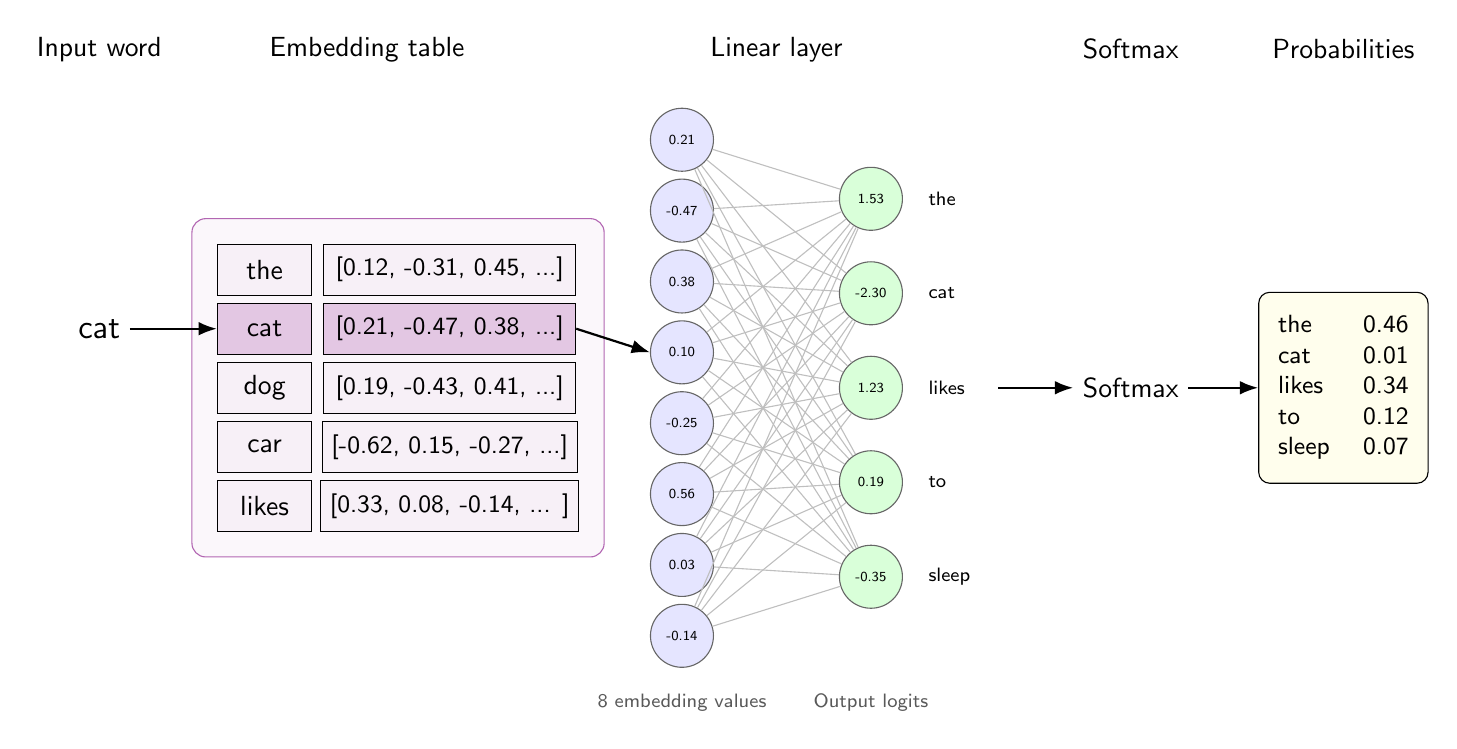
\begin{tikzpicture}[
    >=Latex,
    font=\sffamily,
    neuron/.style={
        circle,
        draw=black!60,
        fill=blue!10,
        minimum size=8mm,
        inner sep=0pt,
        font=\sffamily\tiny
    },
    output/.style={
        circle,
        draw=black!60,
        fill=green!15,
        minimum size=8mm,
        inner sep=0pt,
        font=\sffamily\tiny
    },
    connection/.style={
        draw=black!25,
        thin
    },
    arrow/.style={
        ->,
        thick
    },
    heading/.style={
        font=\sffamily,
        anchor=center
    }
]

% --------------------------------------------------
% Headings
% --------------------------------------------------

\node[heading] at (0,4.3) {Input word};
\node[heading] at (3.4,4.3) {Embedding table};
\node[heading] at (8.6,4.3) {Linear layer};
\node[heading] at (13.1,4.3) {Softmax};
\node[heading] at (15.8,4.3) {Probabilities};

% --------------------------------------------------
% Input word
% --------------------------------------------------

\node[font=\sffamily\large]
    (input) at (0,0.75) {cat};

% --------------------------------------------------
% Embedding lookup table
% --------------------------------------------------

\foreach \i/\y/\word/\values in {
    1/1.5/the/{0.12, -0.31, 0.45, ...},
    2/0.75/cat/{0.21, -0.47, 0.38, ...},
    3/0/dog/{0.19, -0.43, 0.41, ...},
    4/-0.75/car/{-0.62, 0.15, -0.27, ...},
    5/-1.5/likes/{0.33, 0.08, -0.14, ...}
}{
    \ifnum\i=2
        \def\rowcolor{violet!22}
    \else
        \def\rowcolor{violet!6}
    \fi

    \node[
        draw,
        fill=\rowcolor,
        minimum width=1.2cm,
        minimum height=0.65cm
    ] (word\i) at (2.1,\y) {\word};

    \node[
        draw,
        fill=\rowcolor,
        minimum width=3.2cm,
        minimum height=0.65cm,
        font=\sffamily\small
    ] (vec\i) at (4.45,\y) {[\values]};
}

% Box around embedding table
\begin{scope}[on background layer]
\node[
    draw=violet!60,
    fill=violet!3,
    rounded corners=5pt,
    inner sep=9pt,
    fit=(word1)(vec1)(word5)(vec5)
] (tablebox) {};
\end{scope}

\draw[arrow] (input) -- (word2.west);

% --------------------------------------------------
% Linear layer: embedding values
% --------------------------------------------------

\foreach \i/\y/\val in {
    1/3.15/0.21,
    2/2.25/-0.47,
    3/1.35/0.38,
    4/0.45/0.10,
    5/-0.45/-0.25,
    6/-1.35/0.56,
    7/-2.25/0.03,
    8/-3.15/-0.14
}{
    \node[neuron] (h\i) at (7.4,\y) {\val};
}

% --------------------------------------------------
% Linear layer: output logits
% --------------------------------------------------

\foreach \i/\y/\val/\word in {
    1/2.4/1.53/the,
    2/1.2/-2.30/cat,
    3/0/1.23/likes,
    4/-1.2/0.19/to,
    5/-2.4/-0.35/sleep
}{
    \node[output] (o\i) at (9.8,\y) {\val};

    \node[
        right=2mm of o\i,
        font=\sffamily\scriptsize
    ] (label\i) {\word};
}

% Embedding to input layer
\draw[arrow] (vec2.east) -- (h4.west);

% Fully connected weights
\foreach \i in {1,...,8}{
    \foreach \j in {1,...,5}{
        \draw[connection] (h\i) -- (o\j);
    }
}

% --------------------------------------------------
% Softmax (no box)
% --------------------------------------------------

\node[font=\sffamily]
    (softmax) at (13.1,0) {Softmax};

% Start arrow AFTER the output word "likes"
\draw[arrow]
    ([xshift=3mm]label3.east) -- (softmax.west);

% --------------------------------------------------
% Probabilities (aligned columns)
% --------------------------------------------------

\node[
    draw,
    rounded corners=4pt,
    fill=yellow!7,
    inner sep=7pt,
    font=\sffamily\small
] (probs) at (15.8,0)
{
    \begin{tabular}{@{}lr@{}}
        the   & 0.46 \\
        cat   & 0.01 \\
        likes & 0.34 \\
        to    & 0.12 \\
        sleep & 0.07
    \end{tabular}
};

\draw[arrow]
    (softmax.east) -- (probs.west);

% --------------------------------------------------
% Annotations
% --------------------------------------------------

\node[
    font=\sffamily\scriptsize,
    text=black!65
] at (7.4,-4.0) {8 embedding values};

\node[
    font=\sffamily\scriptsize,
    text=black!65
] at (9.8,-4.0) {Output logits};

\end{tikzpicture}

\end{document}

